%%%%%%%%%%%%%%%%%%%%%%%%%%%%%%%%%%%%%%%%%%%%%%%%%%%%%%%%%%%%%%%%%%%%%%%%%%%%%%%%%
%																				%
%                                ELEN4020.tex    			    				%
%						    	Emma Clark(1088496) 							%
%                               Jason Smit (709363)		        				%
%						      Isabel Tollman (728359)           				%
%                                                                   		    %
%                                                                               %
%																				%
%%%%%%%%%%%%%%%%%%%%%%%%%%%%%%%%%%%%%%%%%%%%%%%%%%%%%%%%%%%%%%%%%%%%%%%%%%%%%%%%%
\documentclass[10pt,onecolumn]{witseiepaper}
\pagenumbering{arabic} %set the style of numbering

\usepackage[none]{hyphenat}
\usepackage{flushend}
\usepackage{rotating} %
\usepackage{url} %for url's in the reference
\usepackage[square,comma,numbers,sort&compress]{natbib} %for referencing very important
\usepackage{balance} %balance the last page
\usepackage{amsmath} %math package
\usepackage{xr} %Reference appendix

% for putting code into the report : Looks really good
%%%%%%%%%%%%%%%%%%%%%%%%%%%%%%%%%%%%%%%%%%%%%%%%%%%%%%%%%%%%%%%%%%%%%%%%%%%%%%%%%
\usepackage{listings} 															%
\usepackage{color} 		%
																				%
\definecolor{dkgreen}{rgb}{0,0.6,0}												%
\definecolor{gray}{rgb}{0.5,0.5,0.5}											%
\definecolor{mauve}{rgb}{0.58,0,0.82}											%
																				%
\lstset{frame=tb,																%
  language=C,																%
  aboveskip=3mm,																%
  belowskip=3mm,																%
  showstringspaces=false,														%
  columns=flexible,																%
  basicstyle={\small\ttfamily},													%
  numbers=none,																	%
  numberstyle=\tiny\color{gray},												%			
  keywordstyle=\color{blue},													%
  commentstyle=\color{dkgreen},													%
  stringstyle=\color{mauve},													%
  breaklines=true,																%
  breakatwhitespace=true,														%
  tabsize=3																		%
}																				%
%%%%%%%%%%%%%%%%%%%%%%%%%%%%%%%%%%%%%%%%%%%%%%%%%%%%%%%%%%%%%%%%%%%%%%%%%%%%%%%%%


		\pdfinfo{
		/Title ()
		/Author (Jason R. Smit)
		/CreationDate (D:201711040830)
		/ModDate (D:201711052000)	
		/Subject (FINAL DRAFT)
		/Keywords ()
		}%needed to put information into a pdf discription file

%%%%%%%%%%%%%%%%%%%%%%%%%%%%%%%%%%%%%%%%%%%%%%%%%%%%%%%%%%%%%%%%%%%%%%%%%%%%%%%

%\usepackage{siunitx}
\usepackage{float}

\renewcommand{\thesection}{\arabic{section}}
\renewcommand{\thesubsection}{\arabic{section}.\arabic{subsection}}
\renewcommand{\thesubsubsection}{\arabic{section}.\arabic{subsection}.\arabic{subsubsection}}

%%%%%%%%%%%%%%%%%%%%%%%%%%%%%%%%%%%%%%%%%%%%%%%%%%%%%%%%%%%%%%%%%%%%%%%%%%%%%%%
\begin{document}
%\begin{titlepage}

\title{\centering \textbf{{ELEN4020 Laboratory 1: Multidimensional array analysis}}}

\author{\centering {{Emma Clark (1088496) \\ Jason Smit (709363) \\ Isabel Tollman (728359)\vspace{4mm}}
{ \\ \normalfont \textit{School of  Electrical \& Information Engineering,}
\textit{University of the
Witwatersrand}\\
Private Bag 3, 2050, Johannesburg, South Africa \\}} \vspace{-6mm}}
%\thanks{School of  Electrical \& Information Engineering. University of the
%Witwatersrand, Private Bag 3, 2050, Johannesburg, South Africa}


%%%%%%%%%%%%%%%%%%%%%%%%%%%%%%%%%%%%%%%%%%%%%%%%%%%%%%%%%%%%%%%%%%%%%%%%%%%%%%%
% 
\abstract{Rank 2 and rank 3 tensor addition and multiplication procedures are discussed. By initially presenting algorithms to perform rank 2 procedures, it becomes clear that those of rank 3 are extensions of the traditional methods used to achieve 2-dimensional addition and multiplication.}

\keywords{Multidimesional tensor, addition, multiplication, pseudo-code, C++ \vspace{-6mm}}


\maketitle
\thispagestyle{empty}\pagestyle{empty}
%\end{titlepage}

%%%%%%%%%%%%%%%%%%%%%%%%%%%%%%%%%%%%%%%%%%%%%%%%%%%%%%%%%%%%%%%%%%%%%%%%%%%%%%%
%

\section{INTRODUCTION} 

To implement 3-dimensional (3-D) array multiplication, an investigation of tensor operations is performed. Tensor operation discussion begins with tensors of rank 2. The pseudo-code developed to achieve rank 2 tensor procedures is presented. 

2-Dimensional (2-D) tensor addition is elaborated on in Section \ref{2Dadd}, while multiplication of 2-D arrays is discussed in Section \ref{2Dmult}. Using the basis of rank 2 tensors, rank 3 tensor operations are demonstrated, and the pseudo-code developed to implement the procedures is presented. 3-D array addition and multiplication are illustrated in Sections \ref{3Dadd} and \ref{3Dmult}, respectively. The pseudo-code of each procedure is used to produce C++ code from which to perform all multidimensional array operations.  


%%%%%%%%%%%%%%%%%%%%%%%%%%%%%%%%%%%%%%%%%%%%%%%%%%%%%%%%%%%%%%%%%%%
\section{2-DIMENSIONAL TENSOR ADDITION} \label{2Dadd}

The addition of two 2-D tensors is congruent to addition of two 2-D matrices. Therefore, element-by-element addition is required to achieve the output 2-D matrix, as shown in Equation~\ref{2d-add-eqn}~\cite{matrix_Add}. Algorithm 1 displays the pseudo-code used to calculate the addition of two N$\times$N matrices. \vspace{-5mm}

\begin{align}
C_{ij} = A_{ij} + B_{ij} \label{2d-add-eqn}
\end{align}

\begin{figure*}
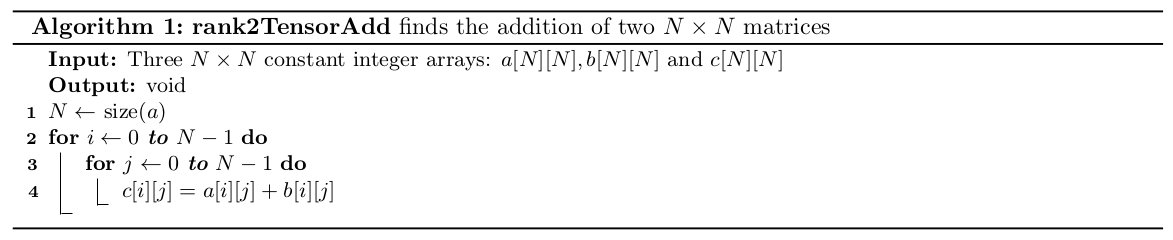
\includegraphics[width=2\columnwidth]{build/Algo1.png}
\caption{Listing showing the pseudo code for Rank 2 addition}
\end{figure*}

%%%%%%%%%%%%%%%%%%%%%%%%%%%%%%%%%%%%%%%%%%%%%%%%%%%%%%%%%%%%%%%%%%%
\section{2-DIMENSIONAL TENSOR MULTIPLICATION} \label{2Dmult}

The multiplication of rank 2 tensors is equivalent to 2-D matrix multiplication, performed by taking the dot product of each row and column, respectively. This is displayed in Equation~\ref{2d-mult-eqn}~\cite{matrix_Multi}. Algorithm 2 shows the pseudo-code used to multiply two N$\times$N matrices. \vspace{-5mm}

\begin{align}
C_{ij} = \sum_{k} A_{ij} \times B_{ij} \label{2d-mult-eqn}
\end{align}

\begin{figure*}
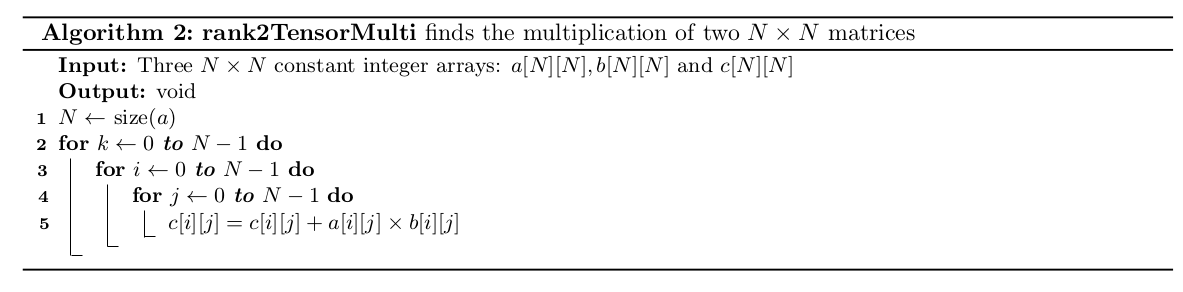
\includegraphics[width=2\columnwidth]{build/Algo2.png}
\caption{Listing showing the pseudo code for Rank 2 multiplication}
\end{figure*}

%%%%%%%%%%%%%%%%%%%%%%%%%%%%%%%%%%%%%%%%%%%%%%%%%%%%%%%%%%%%%%%%%%%
\section{3-DIMENSIONAL TENSOR ADDITION} \label{3Dadd}

Rank 2 tensor addition, discussed in Section \ref{2Dadd}, is used as a basis for 3-D array addition. Algorithm~1 is extended to produce Algorithm~3, applicable for rank 3 tensor addition. When a third rank is incorporated, array addition follows the same procedure as presented in Algorithm~1, however, the additional rank corresponds to an additional vertex of summation.

Element-by-element addition is implemented in a similar fashion to the 2-D array procedure. The difference comes from the inclusion of the additional dimension. Figure \ref{fig:3Dadd} graphically depicts 3-D tensor addition, while Algorithm~3 shows the pseudo-code used to sum two N$\times$N$\times$N matrices. \vspace{3mm}

\begin{figure*}
	\centering
	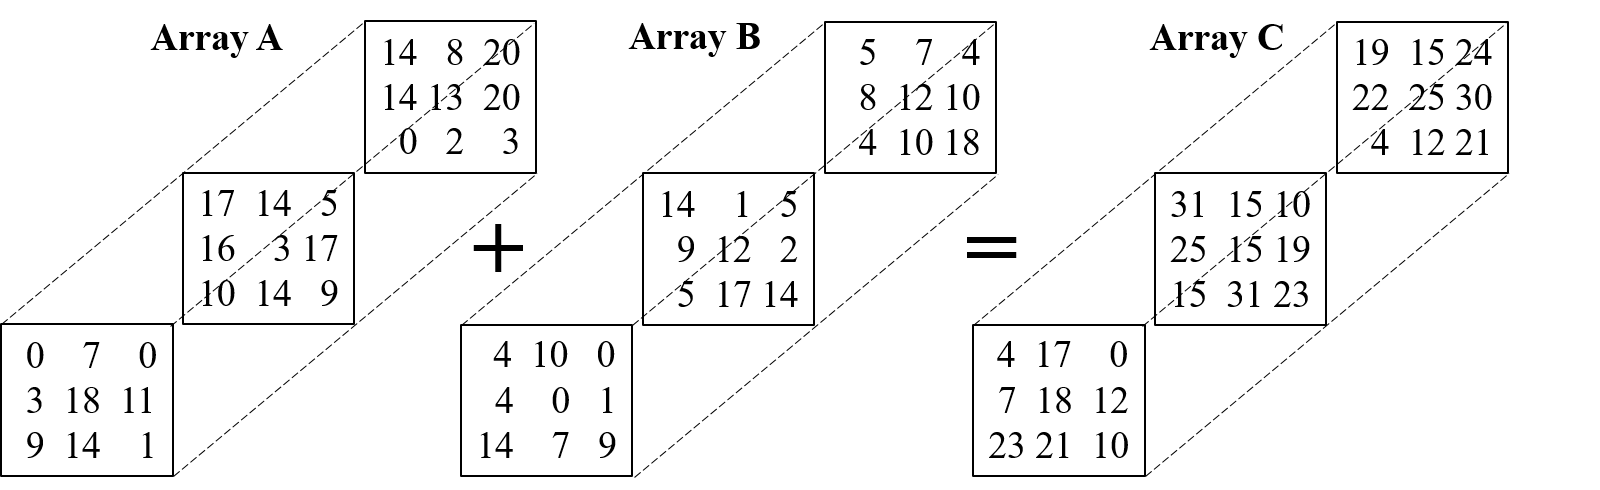
\includegraphics[width=2\columnwidth]{build/AdditionDiagram_3D.png}
	\vspace{3mm}
	\caption{Visualisation of rank 3 tensor addition}
	\label{fig:3Dadd}
\end{figure*}

\begin{figure*}
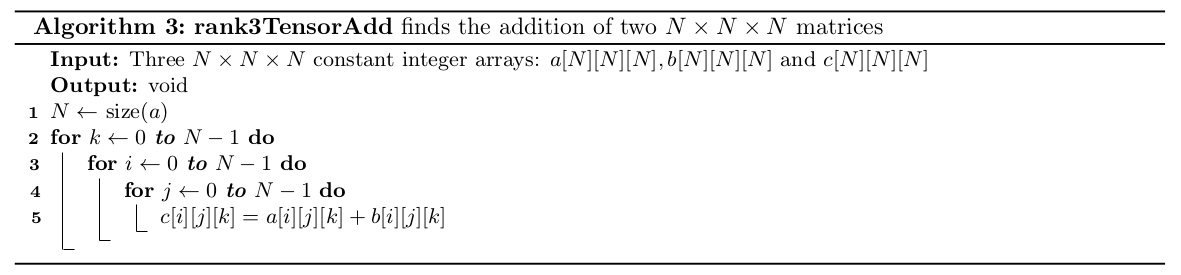
\includegraphics[width=2\columnwidth]{build/Algo3.png}
\caption{Listing showing the pseudo code for Rank 3 addition}
\end{figure*}

%%%%%%%%%%%%%%%%%%%%%%%%%%%%%%%%%%%%%%%%%%%%%%%%%%%%%%%%%%%%%%%%%%%
\section{3-DIMENSIONAL TENSOR MULTIPLICATION} \label{3Dmult}

The multiplication of two 3-D arrays (rank 3 tensor contraction) uses 2-D matrix multiplication as a basis. The $\text{i}^\text{th}$~row-plane of array A and the $\text{j}^\text{th}$~column-plane of array B are multiplied using traditional 2-D matrix multiplication shown in Algorithm~\ref{2d-mult-eqn}. The result is the $\text{k}^\text{th}$ layer-plane of array C. Algorithm 4 provides the pseudo-code used to multiply two N$\times$N$\times$N arrays. Figure \ref{3D} illustrates the implemented algorithm.

\begin{figure*}
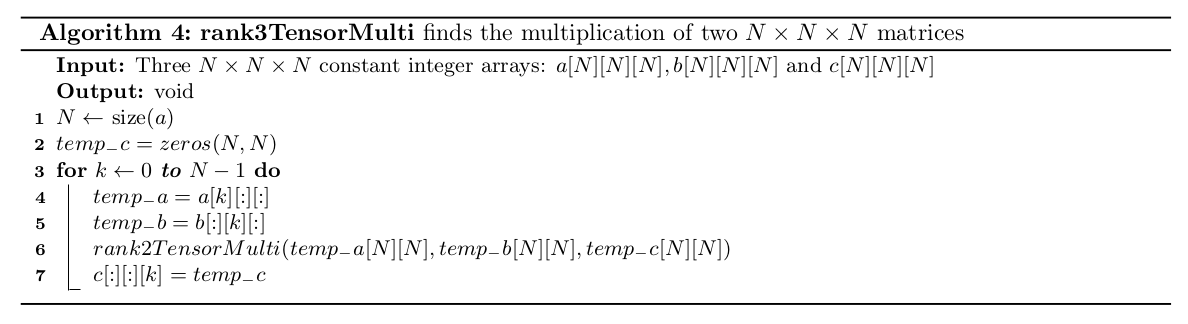
\includegraphics[width=2\columnwidth]{build/Algo4.png}
\caption{Listing showing the pseudo code for Rank 3 multiplication}
\end{figure*}

\begin{figure*}
	\centering
	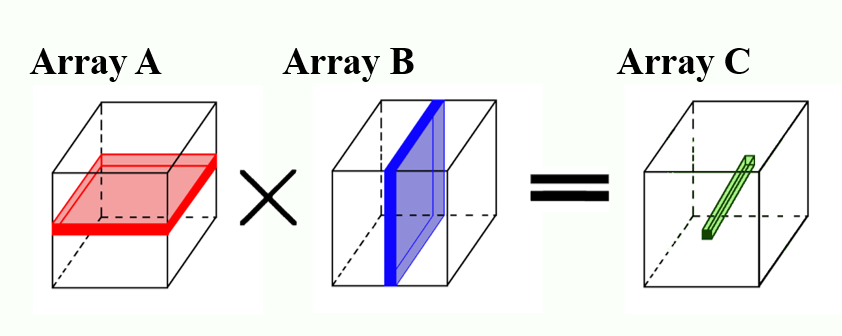
\includegraphics[scale=0.5]{build/3Dmult.png}
	\caption{Visualisation of rank 3 tensor multiplication}
	\label{3D}
\end{figure*}

%%%%%%%%%%%%%%%%%%%%%%%%%%%%%%%%%%%%%%%%%%%%%%%%%%%%%%%%%%%%%%%%%%%
\section{IMPLEMENTATION}

The algorithms presented in Sections \ref{2Dadd}, \ref{2Dmult}, \ref{3Dadd}, and \ref{3Dmult} are implemented using C++. The generated code performs as detailed by the pseudo-code. One .cpp file exists. It is accessible via the public GitHub repository found through link \url{https://github.com/IsabelTollman/ELEN4020A_Group7/tree/Code} under the `\emph{Code}' branch and within the \textit{Code} folder.

%%%%%%%%%%%%%%%%%%%%%%%%%%%%%%%%%%%%%%%%%%%%%%%%%%%%%%%%%%%%%%%%%%%%%%%%%%%%%%%%
\section{CONCLUSIONS}

The formation of rank 3 tensor operations is based on the widely known traditional rules of rank 2 tensors. Rank 3 tensor addition requires a further iteration than 2-D tensor addition. 3-D by 3-D array multiplication uses the procedure of rank 2 tensor multiplication while incorporating the additional dimension through an extra iteration. 

%\cite{1}
 
%%%%%%%%%%%%%%%%%%%%%%%%%%%%%%%%%%%%%%%%%%%%%%%%%%%%%%%%%%%%%%%%%%%%%%%%%%%%%%%
%\clearpage %On a newpage
%\onecolumn
\bibliographystyle{witseie}
\bibliography{build/bibliography_lab1_app}

%{\tiny \vfill \hfill \today \hspace{5mm} witseie-paper-2003.\TeX}


%%%%%%%%%%%%%%%%%%%%%%%%%%%%%%%%%%%%%%%%%%%%%%%%%%%%%%%%%%%%%%%%%%%%%%%%%%%%%%%%%%%%%%%%%%%%%%%%%%%%%%%%%%%%%%%%%%%%%%%%%%%%%%%%%%%%%%%%%%%
\end{document}

" vim: ts=4
" vim: tw=78
" vim: autoindent
" vim: shiftwidth=4
